\documentclass[10pt,xcolor=pdflatex]{beamer}
\usepackage{newcent}
\usepackage[utf8]{inputenc}
\usepackage[slovak]{babel}
\usepackage{hyperref}
\usepackage{fancyvrb}
\usetheme{FIT}

\title[Time Tracker]{Obhajoba projektu -- Time Tracker}

\author[]{\small Dávid Bolvanský, Martin Marušiak, Juraj Ondrej Dúbrava}

\institute[]{}

\date{\today}

\begin{document}

\frame[plain]{\titlepage}

\begin{frame}
\frametitle{Body obhajoby}
\begin{itemize}
	\item Definícia problému
	\item Naše riešenie
	\item Implementácia programu
	\item Užívateľské testovanie
\end{itemize}
\end{frame}


\begin{frame}
\frametitle{Užívatelia a definícia problému}
\begin{itemize}
	\item Užívatelia: študenti, ľudia v~produktívnom veku, ktorí trávia veľa času na PC
	\item Chcú byť efektívnejší, radi plánujú.
	\item Pri práci na PC, často strácajú prehľad o~čase, sú rozptyľovaní, dochádza k~odklonu od plánu.
	\item Plán dňa majú premyslený len v~hlave, prípadne poznačený bokom na papieri, kontrola záleží len na nich, na plán často zabudnú.
	\item Pri pláne na papier často používajú niekoľko rôznych útržkov, na každom útržku sú len veci, ktoré spolu súvisia, radi kategorizujú.
	\item Na konci dňa si vyhradia chvíľu a zamyslia sa nad tým, aký bol ich deň, čo sa im podarilo a čo nie.
\end{itemize}
\end{frame}

\begin{frame}
	\frametitle{Nevýhody existujúcich riešení}
	\begin{itemize}
		\item Ako webová aplikácia:
			\begin{itemize}
				\item[--] nutnosť pripojenia k~internetu, stabilita pripojenia
				\item[--] kompatibilita webovej stránky s~prehliadačmi
				\item[--] slabá (žiadna) interakcia s~jadrom OS (obmedzené sandboxom prehliadača)
				\item[--] bez podpory klávesových skratiek
			\end{itemize}
		\item Ako desktopová aplikácia:
		\begin{itemize}
			\item[--] naviazanosť na konkrétne desktopové rozhranie (DE)
			\item[--] horšia (žiadna) podpora viacerých OS
			\item[--] zastaranosť použitých technológií, slabá rozšíriteľnosť programu
		\end{itemize}
	\end{itemize}
\end{frame}

\begin{frame}
	\frametitle{Naše riešenie}
	\begin{itemize}
		\item[+] \uv{it just works} -- žiadne zložité nastavovanie pri spustení programu
		\item[+] nezávislosť fungovania programu od pripojenia k~internetu
		\item[+] podpora behu na viacerých OS (Linux, Windows) bez obmedzení vo funkcionalite programu
		\item[+] rovnaký dizajn grafického rozhrania na rôznych OS
		\item[+] podpora klávesových skratiek
		\item[+] \uv{search as you type} vyhľadávanie nad zoznamom aktivít
		\item[+] komunikácia s~jadrom systému (sledovanie spustených programov)
		\item[+] aktuálne technológie C++ a Qt/QML, architektúra MVC
		\item[+] i18n, bezplatné, open source
	\end{itemize}
\end{frame}

\begin{frame}
	\frametitle{Prototyp GUI}
	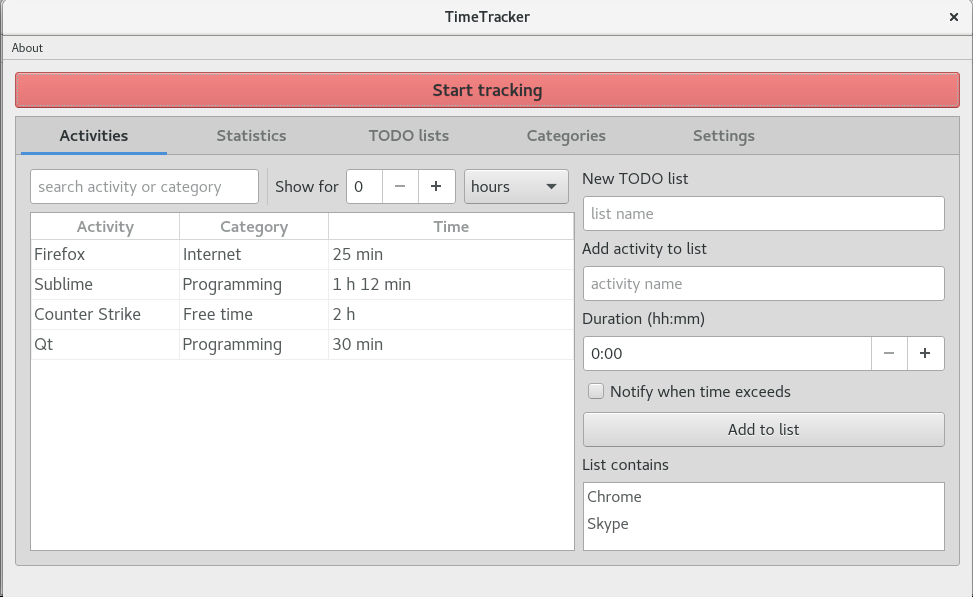
\includegraphics[width=11cm, height=7cm]{prototyp_gui}
\end{frame}



\begin{frame}
	\frametitle{Domovská obrazovka}
	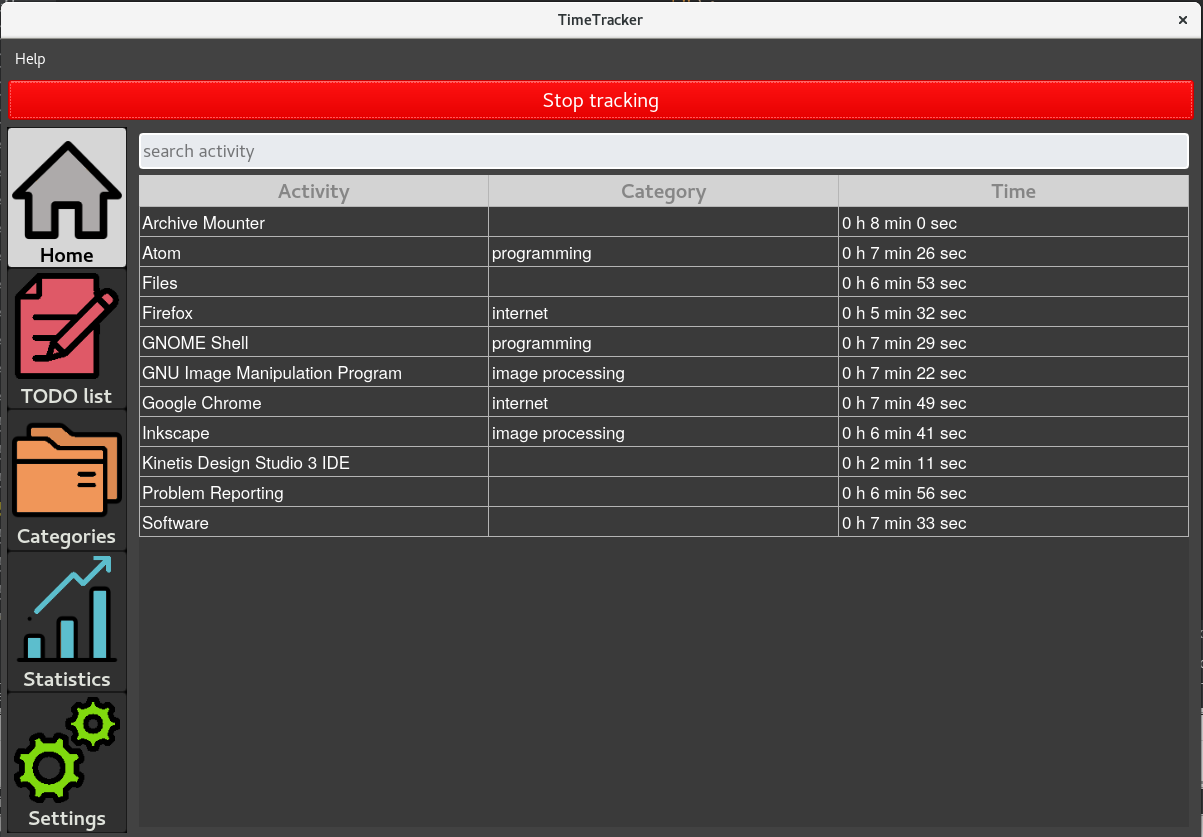
\includegraphics[width=11cm, height=7cm]{mainwindow}
\end{frame}

\begin{frame}
\frametitle{TODO listy}
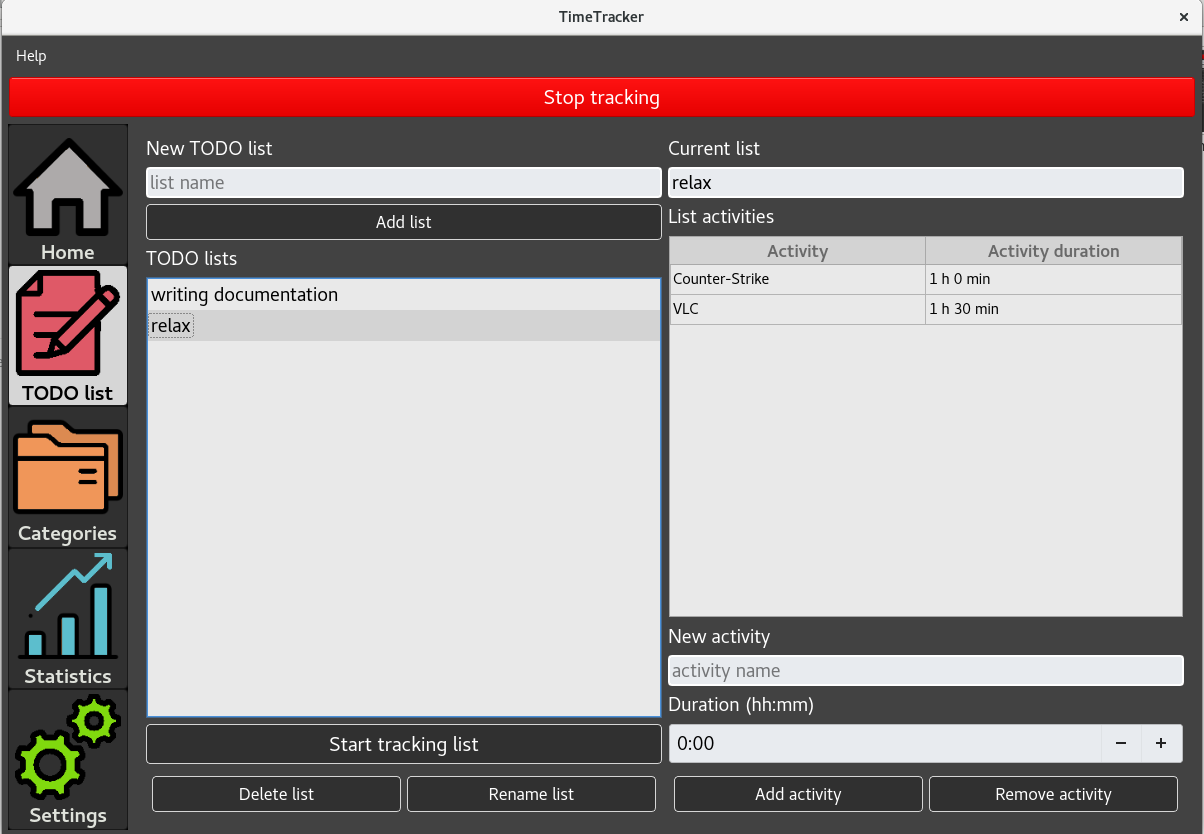
\includegraphics[width=11cm, height=7cm]{todo_list}
\end{frame}

\begin{frame}
\frametitle{Kategórie}
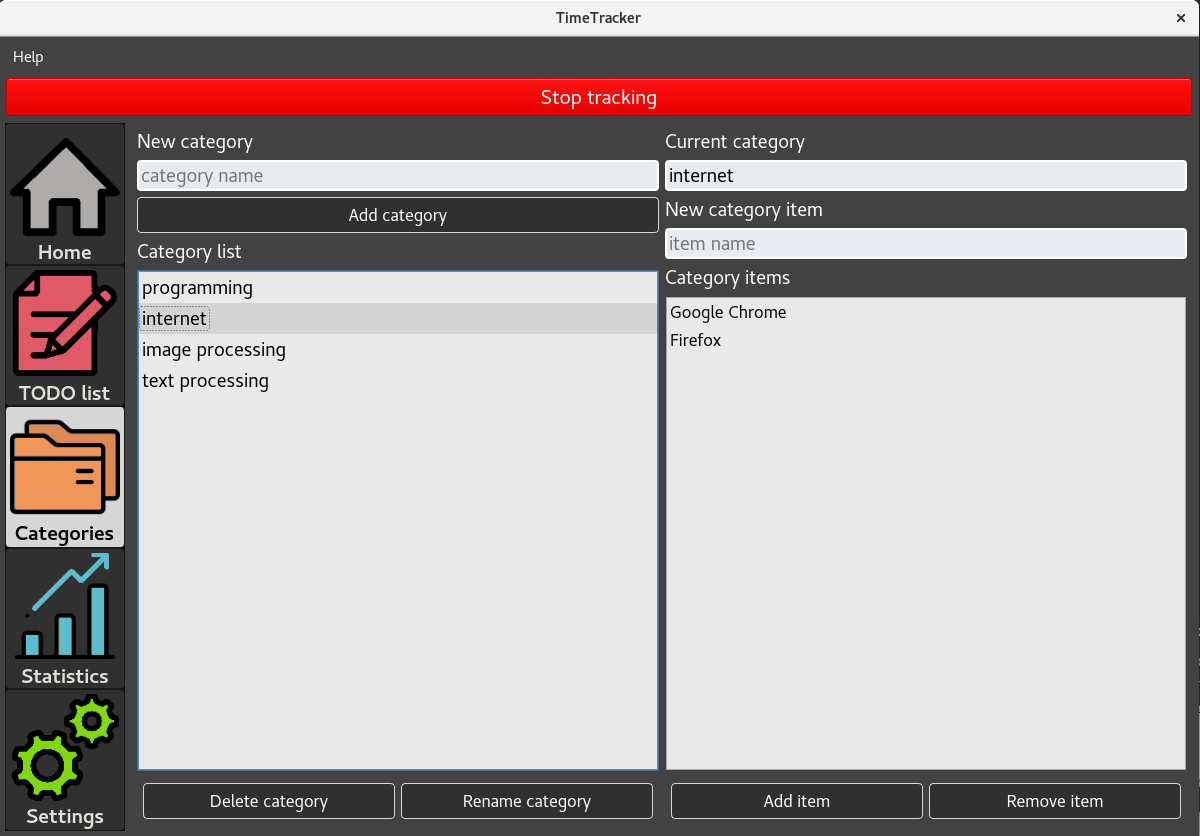
\includegraphics[width=11cm, height=7cm]{categories}
\end{frame}

\begin{frame}
\frametitle{Štatistiky}
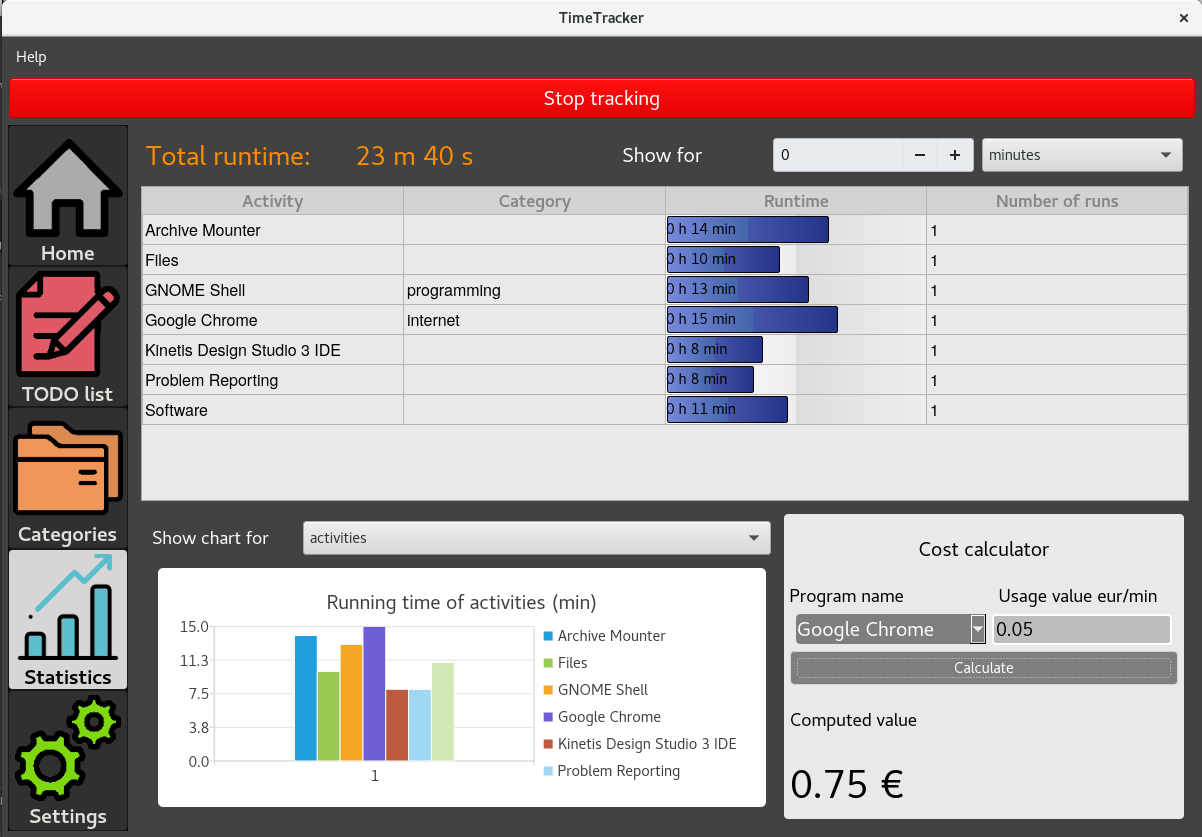
\includegraphics[width=11cm, height=7cm]{statistics}
\end{frame}

\begin{frame}
\frametitle{Nastavenia}
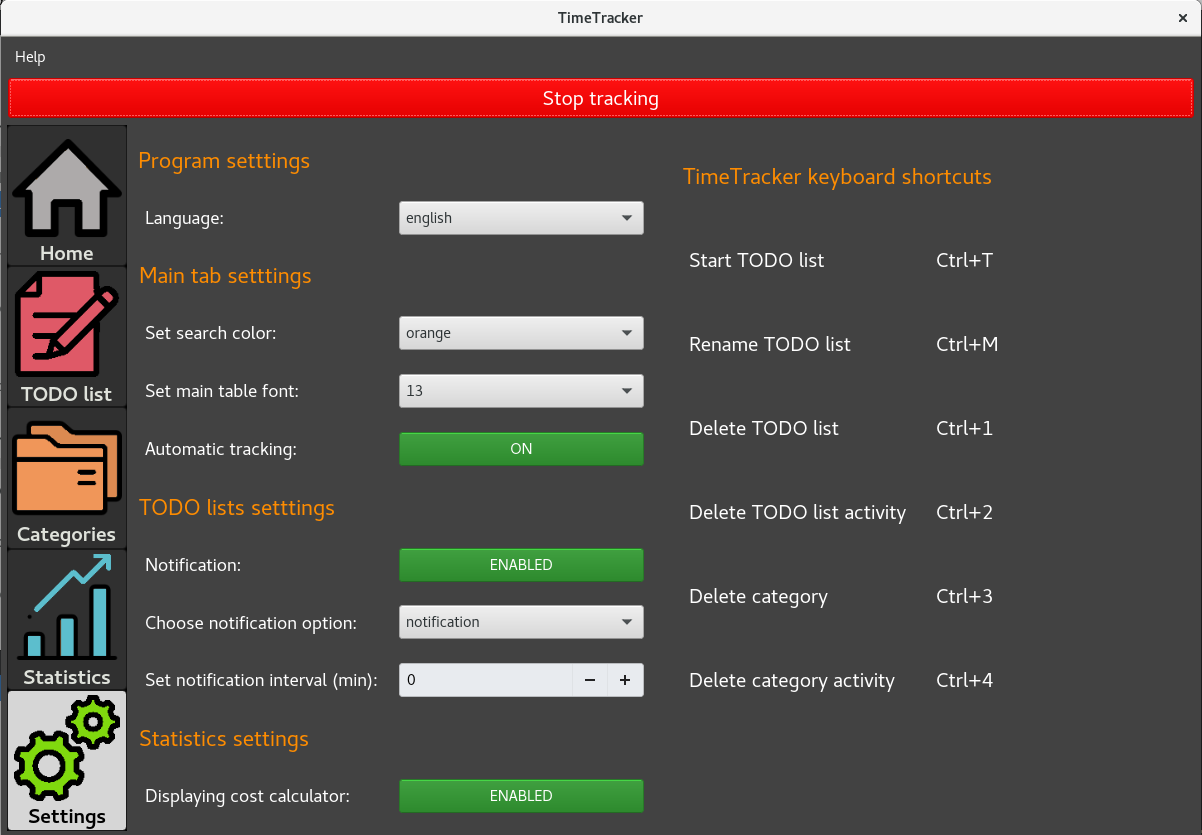
\includegraphics[width=11cm, height=7cm]{settings}
\end{frame}

\begin{frame}
	\frametitle{Užívateľské testovanie}
	\begin{itemize}
		\item uskutočnené v~záverečných fázach vývoja produktu
		\item 4 osoby vo veku 19 až 24 rokov, 3 muži a 1 žena
		\item priame pozorovanie
		\item protokol hlasného myslenia
		\item zoznam úloh na vykonanie, oddelené testovanie
		\item výsledky užívateľského testovania $\rightarrow$ identifikácia problémov:
		\begin{itemize}
			\item nejasné vyhľadávanie aktivít
			\item dlhý čas odozvy od začiatku vyhľadávania po zmenu v~ grafickom rozhraní
			\item komplikované riešenie premenovania TODO listov a kategórií
		\end{itemize}
		\item eliminácia zistených problémov $\rightarrow$ zmeny v~GUI
	\end{itemize}
\end{frame}

\begin{frame}
\frametitle{Time Tracker}
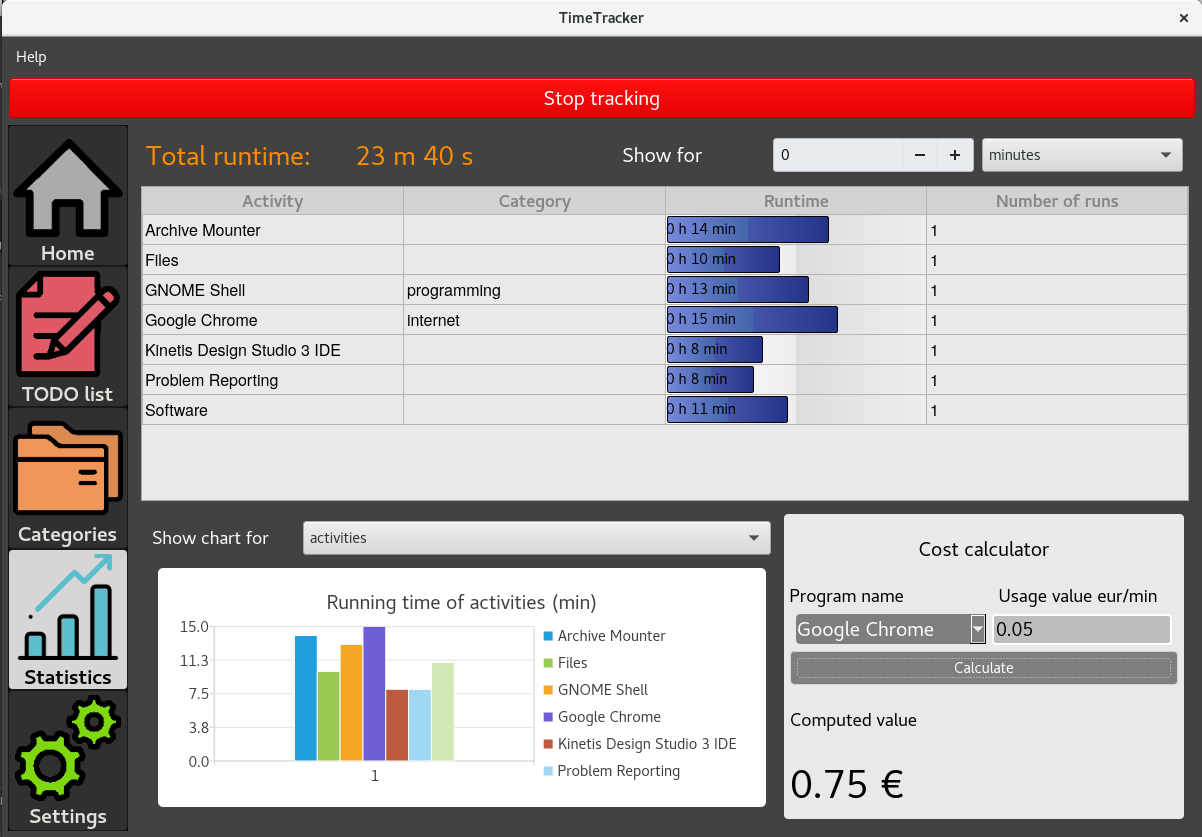
\includegraphics[width=11cm, height=7cm]{statistics}
\end{frame}

\end{document}
